

\begin{figure}[!htb]
     {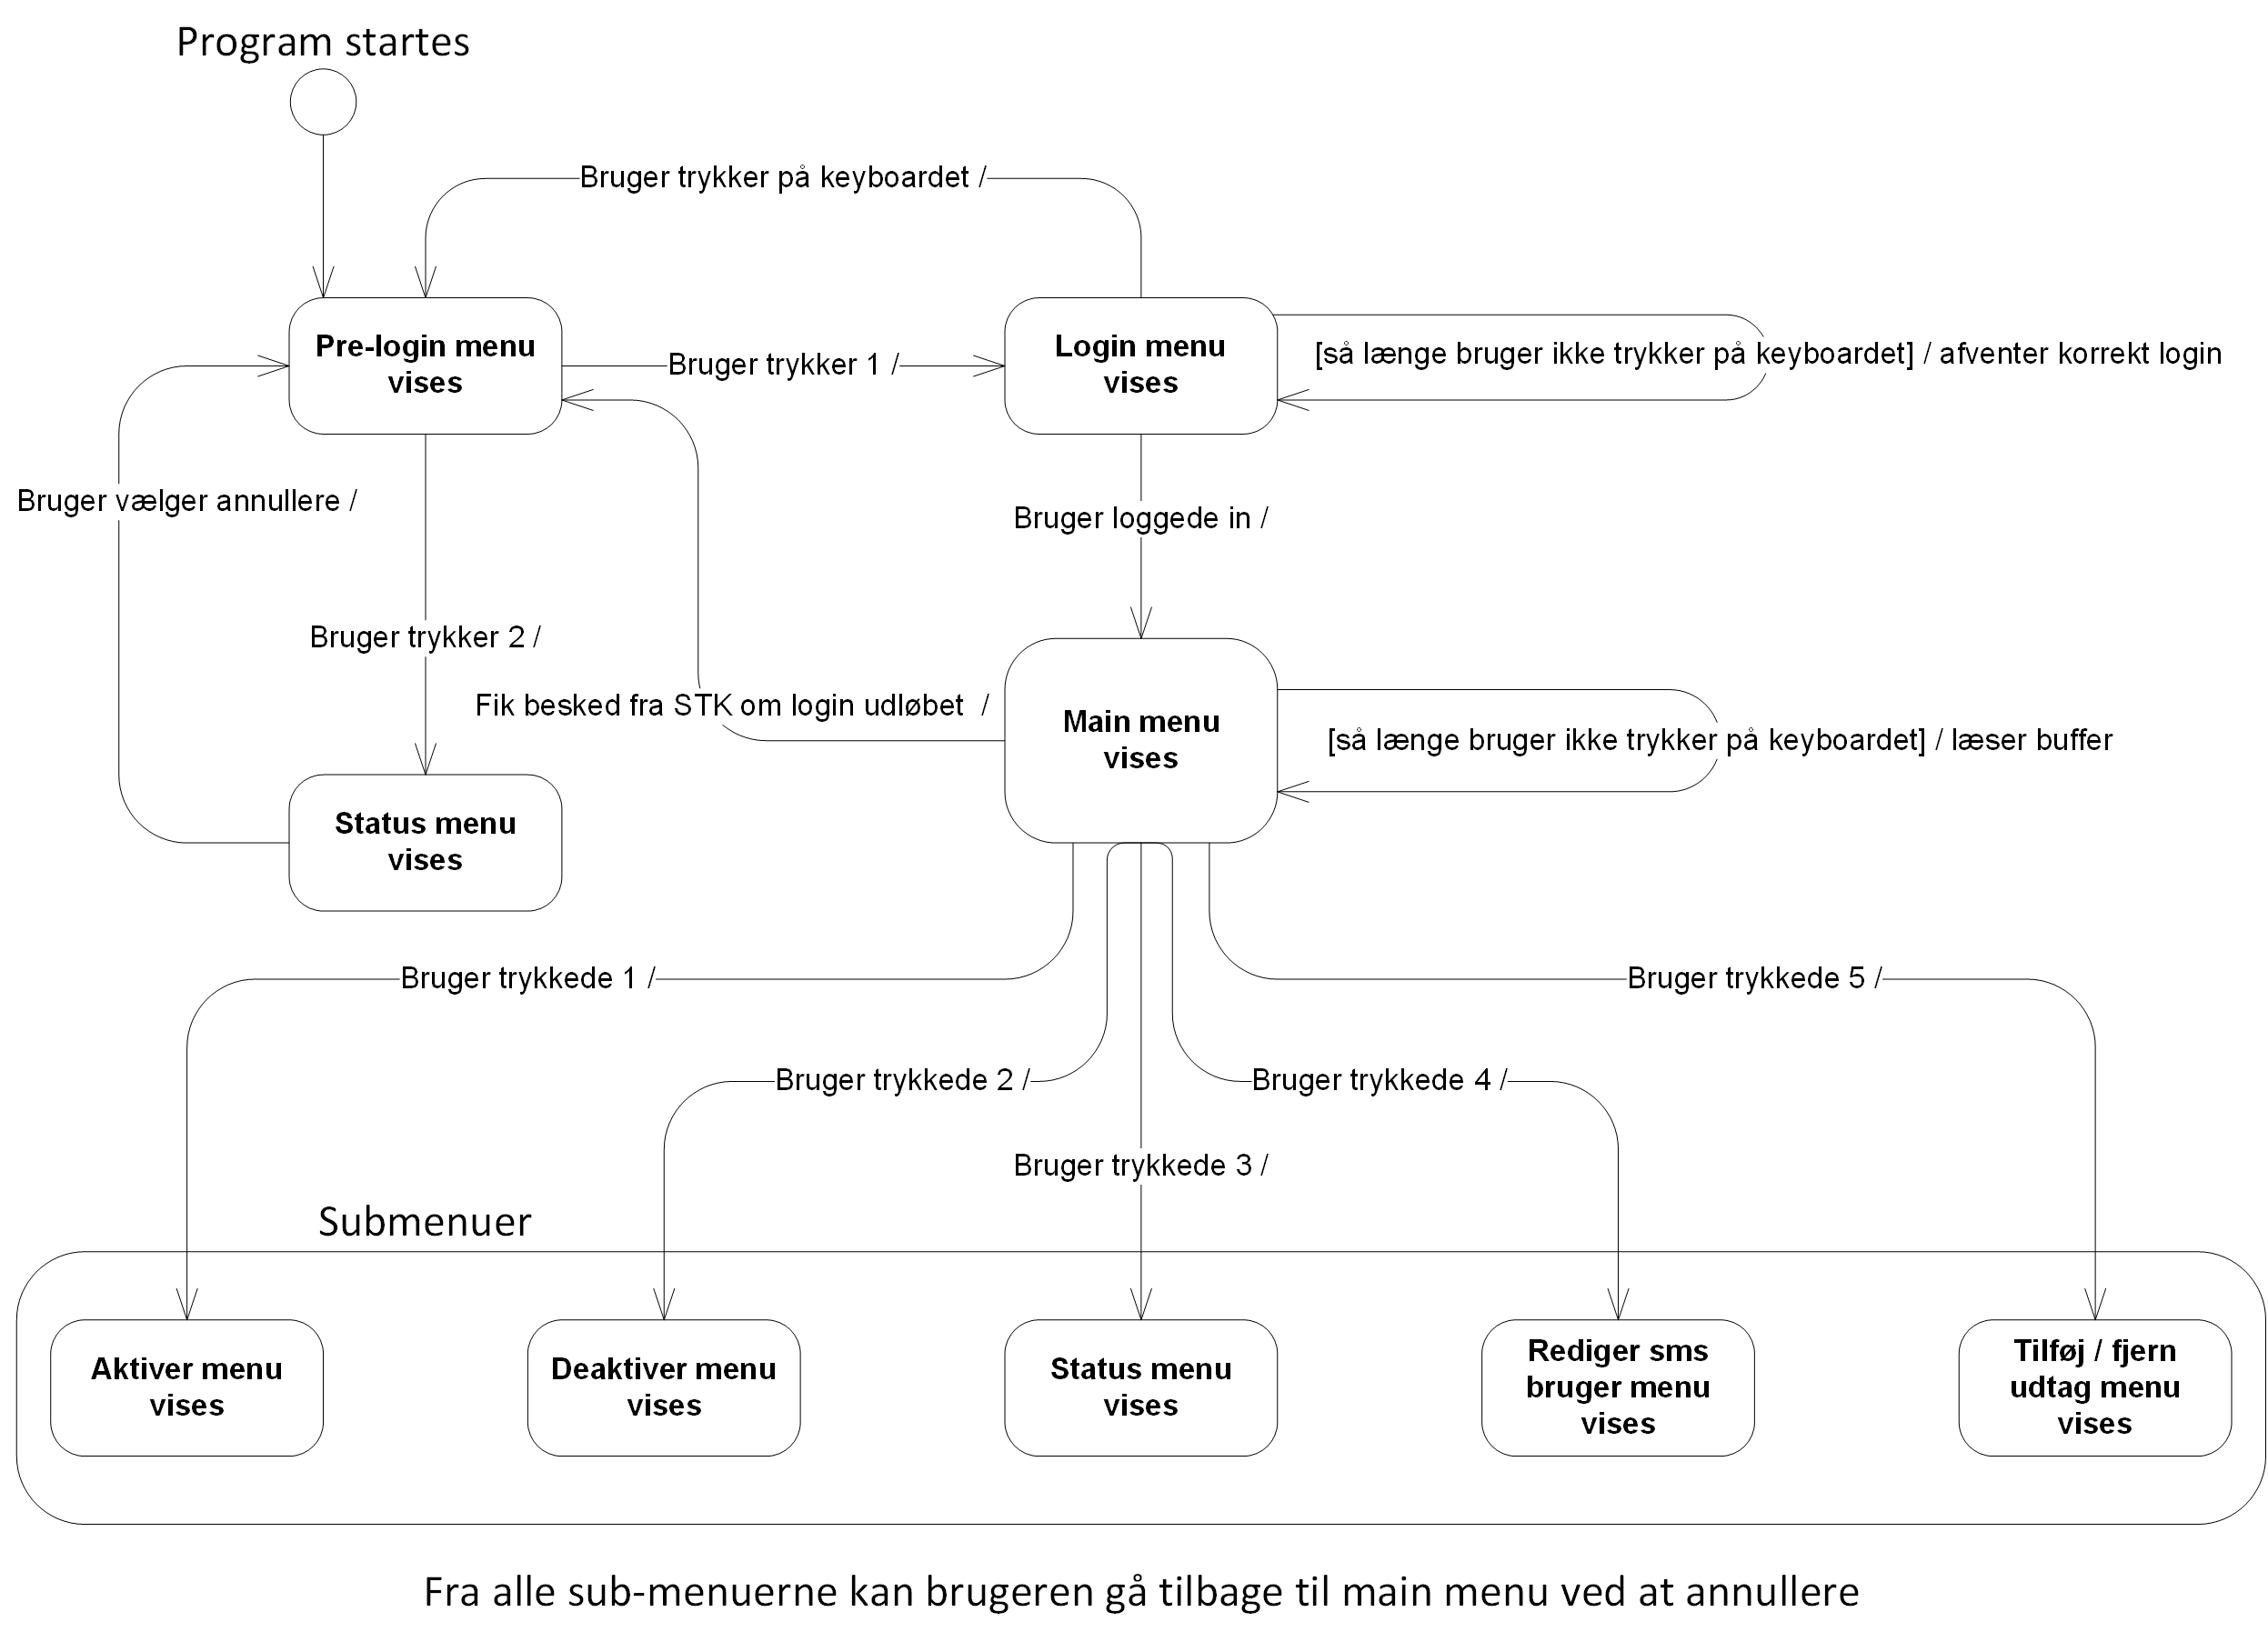
\includegraphics[width=\textwidth]{billeder/uml/state_machine_main}}
     \caption{State machine diagram over forløbet fra PC start til menuer.}
     \label{fig:State_machine_pc}
\end{figure}

Diagrammet ovenfor skal illustrere hvordan forløbet er fra PC opstart. Hvor man møder Pre-login menuen som kun giver en mulighed for at få vist login menu eller vis status menu. Efter der er logget ind vil den stå og føle på input bufferen, på den port hvor PC'en er forbundet med CSS hovedenheden. Det gør den for at en evt. babyalarm kan afbryde forløbet og blive sendt. Desuden kan CSS hovedenheden give besked om at der ikke længere er logget ind, hvilket sender brugeren til pre-login menuen igen.

\medskip

Når brugeren så trykker på en tast og trykker enter vil han blive sendt til en af de 5 menuer. Dog stadig under forudsætning af at han valgte en værdi imellem 1-5 for den pågældende menu. Ved forkert tast sker der ingenting. Fra hver af de 5 sub-menuer har bruger mulighed for at annullere og komme tilbage til main menuen. Dette gør han ved at taste 27 og enter.


\clearpage

\begin{figure}[!htb]
     {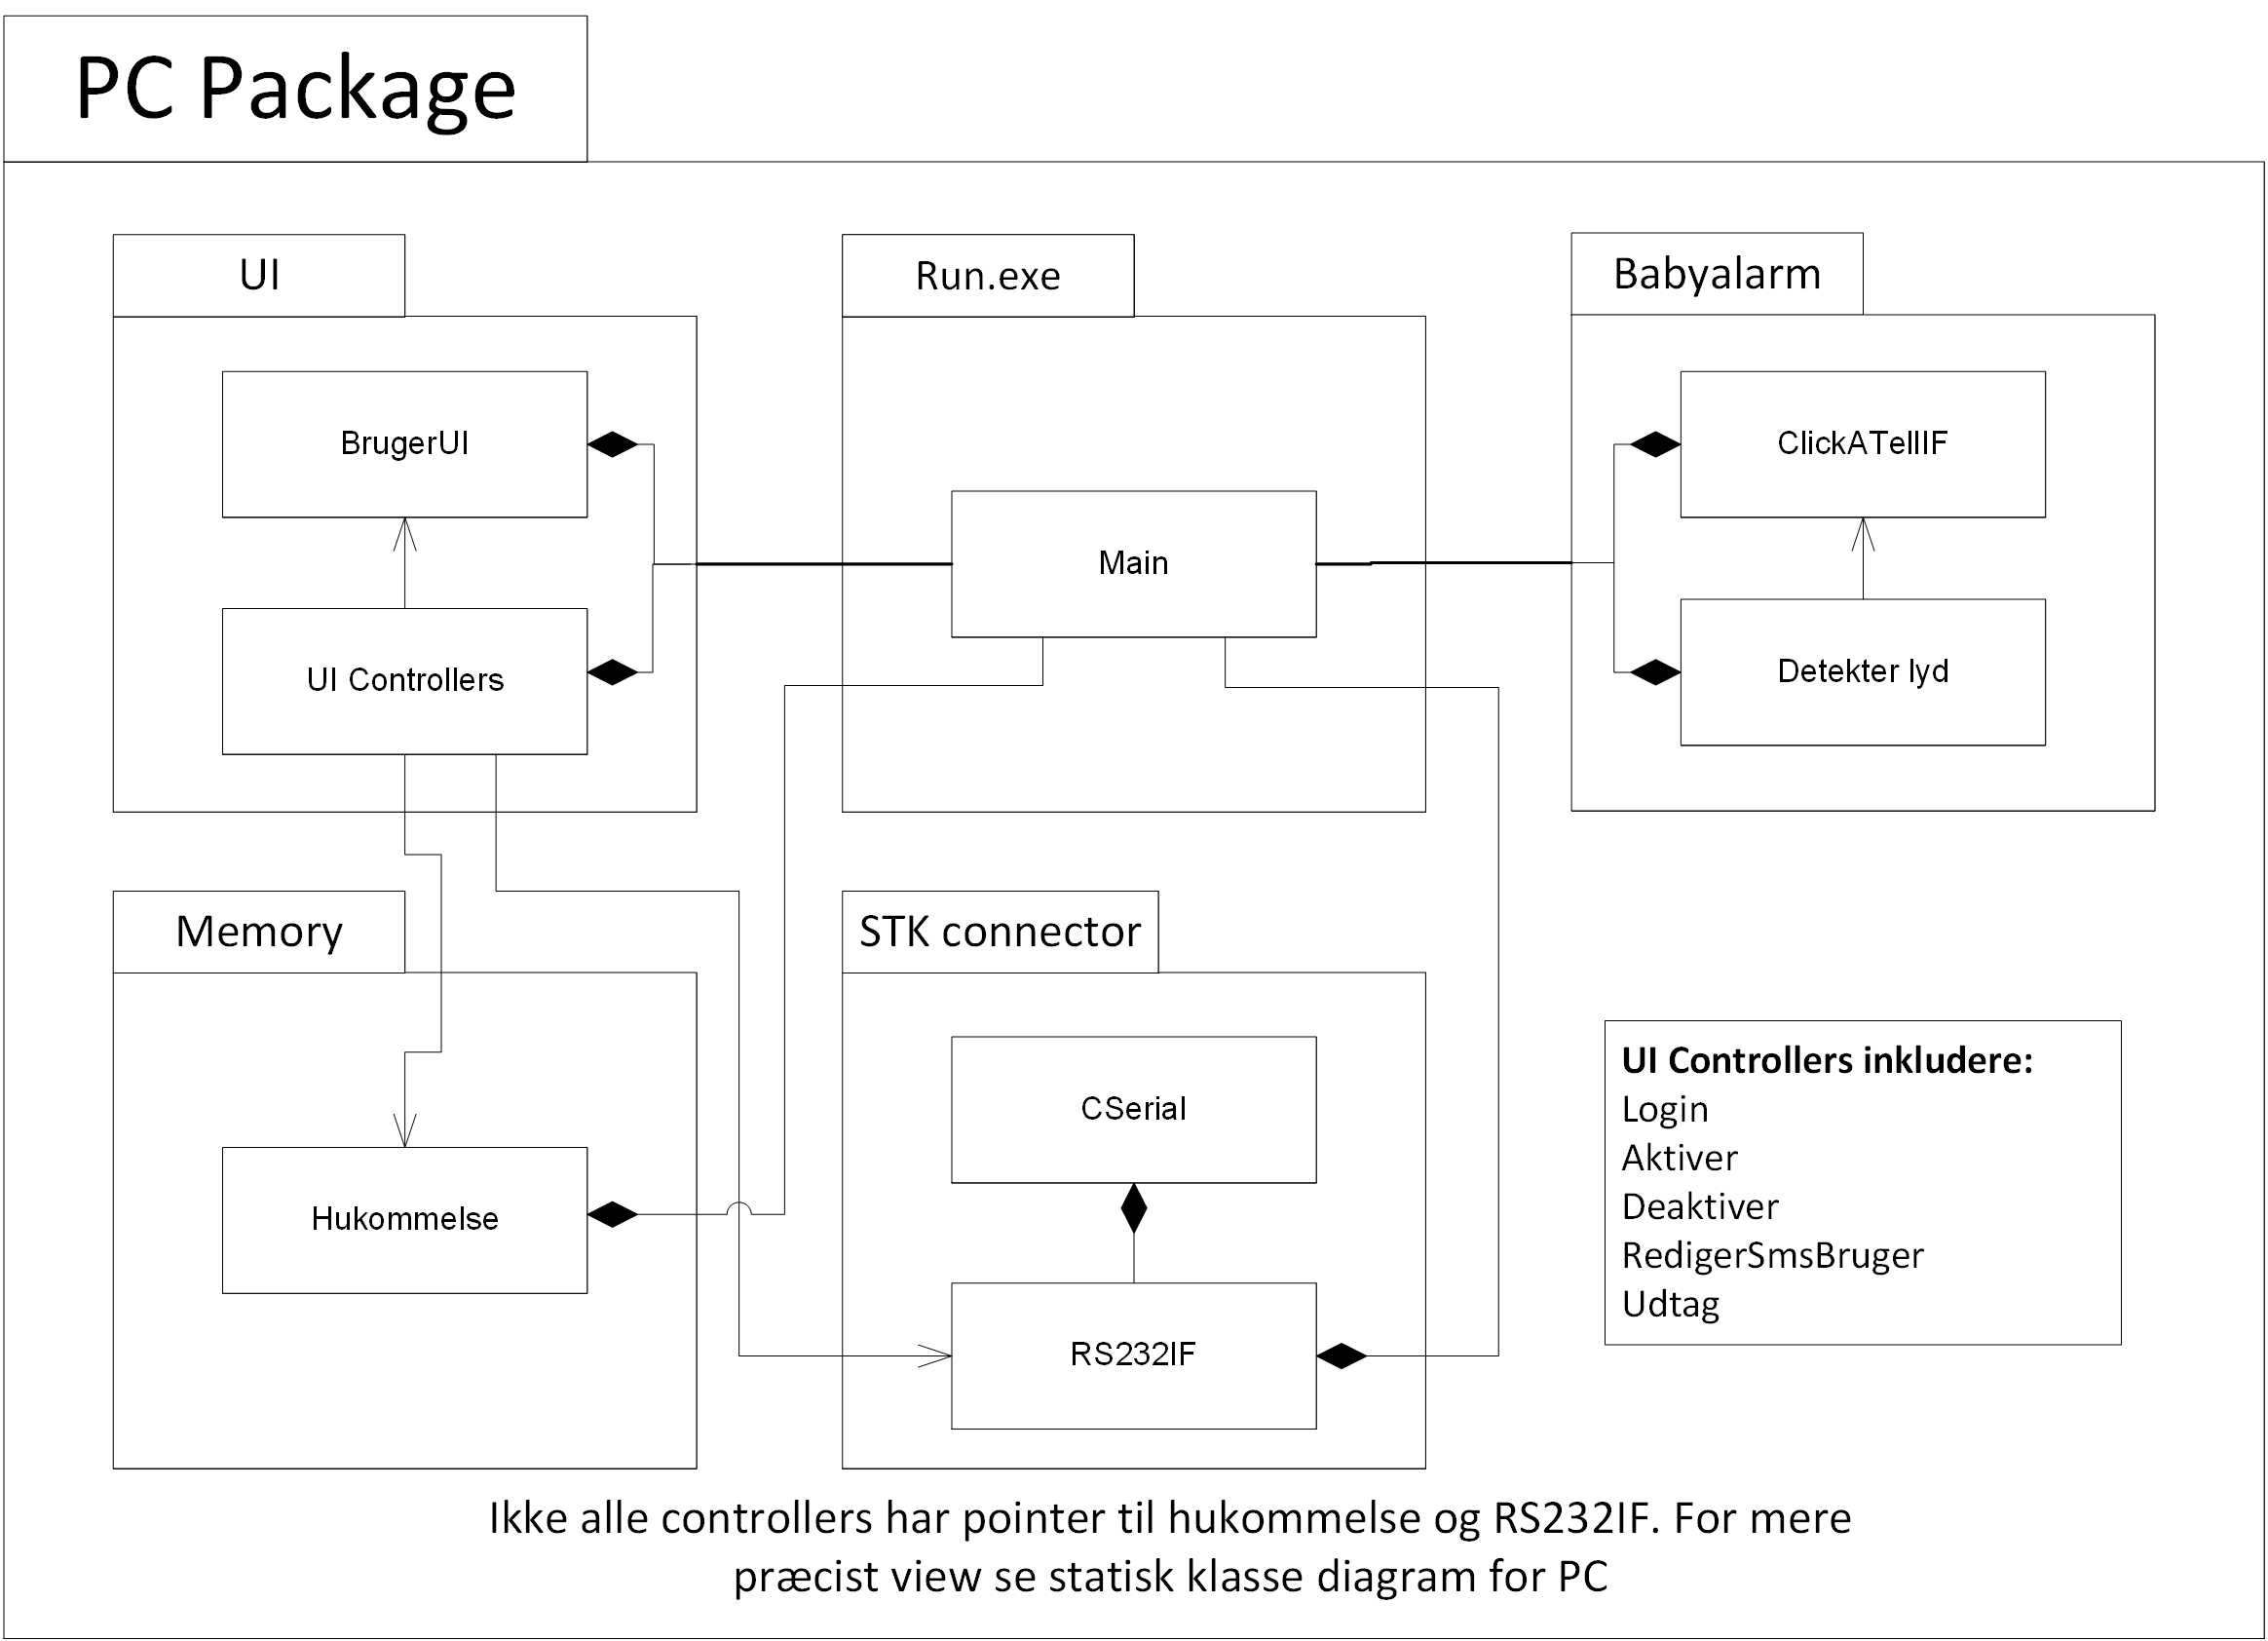
\includegraphics[width=\textwidth]{billeder/uml/logical_view_pc}}
     \caption{Logical view: PC package}
     \label{fig:PC_package}
\end{figure}

Figuren ovenfor viser de forskellige packages man kan indlede PC klasserne i. Alle controllers som har UI pointers er smidt i UI packagen sammen med BrugerUI. STK Connector packagen indeholder RS232IF og så har den et CSerial objekt som er en klasse der har de 5 mest basale metoder til at sende og læse på en seriel port.